\documentclass{CRPITStyle} 
%\usepackage{epsfig}   % Packages to use if you wish
%\usepackage{lscape}   % 
\usepackage[authoryear]{natbib}

\usepackage{ifpdf}
\usepackage[utf8]{inputenc}
\usepackage{cite}
\usepackage{paralist}
\usepackage[pdftex]{graphicx}
\usepackage{caption}
\usepackage{subcaption}
\graphicspath{{.}{images/}} 
\DeclareGraphicsExtensions{.jpg}
\usepackage[cmex10]{amsmath}
\usepackage[rgb]{xcolor}


\newcommand*{\bd}[1]{\multicolumn{1}{|c|}{\bfseries #1}}
\renewcommand{\cite}{\citep}
\pagestyle{empty}
\thispagestyle{empty}
\hyphenation{roddick}

\begin{document}

\title{Securing WSN update from Intrusion using Time Signature of Over the Air Update Protocol}
\author{A S M Ashraful Alam  \and  David Eyers 	  }
\affiliation{Department of Computer Science, University of Otago, New Zealand\\
			Email:~{\tt \{aalam, dme\}@cs.otago.ac.nz} 	}

\maketitle

\newcommand\conferencenameandplace{Twenty-Ninth Australasian Computer Science Conference (ACSC2006), Hobart, Australia}
\newcommand\volumenumber{48}
\newcommand\conferenceyear{2006}
\newcommand\editorname{Vladimir Estivill-Castro and Gillian Dobbie}
\toappearstandard 

\begin{abstract}
While over the air (OTA) software update makes certain WSN management tasks easy, they also remain vulnerable to intrusion attempts.
An adversary can take advantage of the resource constrained nature of the sensor motes and employ enough resources to break in through the limited protection the sensors are armed with.
To deal with this problem, we have suggested a passive security mechanism---an IDS that works on a timing analysis principle.  
\end{abstract}
\vspace{.1in}

\noindent {\em Keywords:} Sensors, Wireless Sensor Network, WSN, IDS, Intrusion Detection System, Security

\section{Introduction}
\label{sec:intro}

Wireless sensors or motes are deployed in large numbers in uncontrolled environments, which makes them difficult to manage.
Requirements such as bug-fixes, altered sensing, are generally managed using over the air (OTA) software update protocols like Deluge~\cite{1031506}.
There are potential dangers associated with Wireless Sensor Network (WSN) OTA software update which can enable an attacker to steal sensitive information, log network events, even complete denial of service.
While OTA update protocols make certain WSN management tasks easy, they also remain vulnerable to intrusion attempts.
An adversary can take advantage of the resource constrained nature of the sensor motes and employ enough resources to break in through the limited protection the sensors are armed with.


Security threats to WSN are different in nature from threats to the Internet or even other wireless technologies. %technology. % and ad-hoc network, MANET.
Implementation of security techniques in WSN are characterised by constrained resources.
Wireless channels are inherently considered to be less secure.
Well developed cryptographic security mechanisms like WPS, PKM and likewise are inappropriate in WSNs.
Moreover, the capability of computing devices that can computationally compromise the cryptographic protection in sensors grows at much faster rate.
As a result, WSNs are more vulnerable to intrusion attempts and security threats from malicious attackers.
In contrast, simple communication protocols and design make it easy to perform intrusion detection in WSN~\cite{quing09}.
An Intrusion Detection System (IDS) can detect  break-in events, and raise alert. % following some predefined procedures. 
It may be able to report the location and extent of break-in as well.


The proposed IDS techniques vary greatly in their ideas and approaches.
Misuse based  detection  techniques aim to detect known attacks by identifying undesired activities based on usage signature.
But they are ineffective against novel attacks and 
may wrongly identify legitimate activities as intrusion because of similarity with the signature.
Conversely, anomaly based IDS builds statistical signature based on defined normal activity.
Unfortunately, a system may display previously unknown behaviour e.g.,rare critical activities like earthquake or tsunami may raise false positive intrusion alert in sensors employed for other environmental monitoring.
On the other hand, an intrusion that masks its pattern under the hood of normal behaviour, for example: increased packet traffic during OTA update, would go undetected.
Specification-based and reputation-based techniques rely on manual input for defining normal and anomalous behaviour with lesser reliance on automation.
However, these techniques also have not been proved to be very effective because human interaction are more prone to errors and require more learning time~\cite{quing09, 1593102, 1290173, Chen:2009:NMI:1516241.1516282}. 
%Although approaches described above
Despite innovative ideas, only few IDSs are able to address the security issues related to software update.

Onat and Miri presented an IDS design in which each node builds an expectation statistics of received packets based on the last N packets received from each neighbour.
If packets received from any neighbour display anomalous patterns after a predefined number of consecutive packets, intrusion alarms may be raised \cite{1512911}.
Unfortunately, the  packet count statistics is not suitable in OTA software update scenario due to significant increase in packet traffic owing to the update process. 
However, the mechanism of statistical treatment on information over a time period motivates us to employ timing analysis approach on the context of OTA update protocol.

In this paper, we present an IDS that can deal with intrusion in case of WSN software update.
The algorithm requires a minor modification of the OTA update protocol to send back a datagram containing the update time, 
which enables the IDS with a centralised view of network-wide knowledge to work out a  `Surprise Score' or `Intrusion Warning Score' (IWS)~\cite{aalam15}.
This work's contributions are two fold: 
\begin{inparaenum}
\item  The IDS identifies anomalies in software update patterns and scores them quantitatively;
\item It is demonstrated that simulation can indicate the positions of WSN nodes that will best support the ability of similar IDSs to detect anomalies. 
%scheme i.e., the IDS expectations can provide useful insight for designing secure WSN.
\end{inparaenum}
The rest of this paper is structured in the following way. 
In Section~\ref{sec:meth}, we describe a brief overview of the system  design and the experiment methodology. 
Then we  present the findings from the experiments, analyse the result and present our evaluation in Section~\ref{sec:eval}.  
Finally, we conclude our arguments in Section~\ref{sec:concl}.


\section{Methodology}
\label{sec:meth}

\subsubsection*{System Design}
%The IDS framework components has been shown in \ref{fig:ids_fw}.
The IDS has three kinds of components --- 
\begin{inparaenum}
\item motes in radio network; 
\item an IDS transport client (ITC) application in the sink; and
\item an IDS application that runs on an system with higher resources, coordinates with ITC, remains physically attached to the sink, and houses a network database (NDB).
\end{inparaenum}
The chronology of the activities in the IDS are ---
\begin{inparaenum}
\item Deluge protocol initiates update;
\item Deluge disseminates the new software image using a multi-hop relay mechanism; 
\item nodes deliver their timing information to the sink using datagram packet;
\item packets from the nodes rely on other nodes enroute to reach to the sink; and
\item the ITC application in the sink delivers relevant information to the IDS for processing 
\end{inparaenum}~\cite{tep116}.
After checking for correctness, the ITC then inserts the update time, mote ID and related information to the network database (NDB) in the IDS.
The IDS maintains an identifier to differentiate among different update times from different runs for the same mote.
The authenticated initial software update runs are considered to be legitimate and the IDS uses these timing measurements to build signature.
The time analyser module in the IDS inspects the NDB once an update activity has been detected and determines the changes from the signature and calculates IWS based on following utility function:
\begin{equation}
\label{eqn2} 
	\mathit{IWS} = \sum \limits_{i=0}^{n} \frac{\left| \mu_i - t_i \right|}{\sigma_i + 1}
\end{equation}
where, 
\begin{inparaenum}
\item $\mathit{i}$---mote index;%\notedme{Why were you using capital letters all through here?} 
\item $\mathit{t_i}$---image update time at mote $\mathit{i}$;  
\item $\mathit{\mu_i}$---mean update time at mote $\mathit{i}$;  
\item $\mathit{\sigma_i}$---standard deviation of update time at mote $\mathit{i}$. 
\end{inparaenum}	


\subsubsection*{Threat Model}
The threat model is directed towards injection of unauthorised program images to infect the entire WSN.
The IDS is expected to handle malicious node update, node compromise, and node failure.
We assume that an  attacker  can take over one or more nodes deployed in hostile environment, access the code in a compromised node, and use cryptanalysis to represent a false identity without physically compromising a node.
However, he has  no special  access to  the  network and is unable to modify the underlying protocols running in the uncompromised nodes.
We assume several settings like static WSN with a single  sink which is  protected from all kinds of attacks and cannot be compromised. All motes are assumed to have time synchronisation accurate to 1~$\mu$s, e.g., achieved using the TSMP. %~\cite{Pister08tsmp:time}.
\subsubsection*{Experiment Settings}
\label{subsec:sim_env} 
We used `Cooja'--a %\footnote{https://github.com/contiki-os/contiki/wiki/An-Introduction-to-Cooja}, a 
 network simulator in Contiki v2.7 running on Ubuntu 12.04, to simulate the software update pattern associated with Deluge protocol.
The simulations evaluated the IDS in different WSN topologies and explored the effect of parameters such as power level.
Evaluating the IDS on each of the topologies consisted of several test runs that  were of two kinds: 
\begin{inparaenum}
\item aimed at building signature consisting of 20 individual simulations initiated from the sink; and
\item simulations that replicated intrusion from different nodes except the sink.
\end{inparaenum}
We explored topologies such as: linear, circular, elliptical, double rings, wide line, grid, tree and other random topologies, but do not have space to describe them all.
The motes were placed at a distance of 30--35 meter to allow  multiple transmission paths to all motes. 
For most experiments, the radio transmission power level was set at 100\% which has an approximate maximum effective transmission range of 50 meters and is able to interfere with other motes up to 100 meters away.
The `Owheo WSN'\footnote{WSN deployed in Department of Computer Science building at the University of Otago. It is intended to be used for research purposes.} topology was additionally tested at 50\% power level.%  to observe the difference from the parameter change.

\subsection*{Procedure}
\label{subsec:proc}

\begin{itemize}
%\subsubsection*{Step 1} 
\item All motes in the WSN were booted up at same time running one version of a diagnostic application that reports its time, version number and mote ID every second on its serial terminal. 
%Step 2: Stopping the simulation
%\subsubsection*{Step 2} 
\item The sink dynamically began the update process by propagating another version of the software image using Deluge protocol. %, which is also called 
Whenever the transfer to a mote was complete, the new image would  reboot to begin executing.
In real system, the suggested modified Deluge protocol that runs with the OS would report the information to the sink using datagram.
The simulator continued until all the motes in the WSN were updated and the reported events were logged. 
The update time of each mote were filtered out  and were sorted In ascending order of update time.
%\subsubsection*{Step 3} 
\item Processed data  were statistically treated to build the signature consisting of mean and standard deviation of  mote update time.
Any change in variable parameters or in the topology setup would necessitate recalibrating the signature.
%\subsubsection*{Step 4} 
\item Intrusion attacks at different nodes were replicated in simulations.
The individual simulations runs were treated in a fashion  similar to~Step 1 and Step 2.
The update time recorded at each of the motes was then analysed using Equation~\ref{eqn2}.
The resulting values from this function presented an approximation of the abnormality of the new update pattern. The higher the score, the more unusual the pattern was. 
%\subsubsection*{Step 5} 
\item We classified IWS into Intrusion Warning Zones (IWZ) based on a scale built from maximum expected IWS for a topology to imply certain warning levels.
The heuristics follows from statistical techniques and feasibility of finding easily identifiable boundary.
The IDS marks an IWS up to 10\% from the scale as GREEN to indicate safe zone,
10\%--30\% as GREY to indicate a situation where rules are not known and 
above 30\% to be possible intrusion and is marked as RED zone.
IWZ depends on the assumed ability of the IDS having IWS knowledge of all possible intrusions in the network.
Such knowledge can be built by replicating intrusion activity from the furthest few nodes.
\end{itemize}

\section{Results and Evaluation}
\label{sec:eval}

\begin{table*}[t!]
\centering
\begin{tabular}{|l|*{19}{r|}r|}
\hline
\bd{Node ID}           & \bd{1} & \bd{2} & \bd{3} & \bd{4} & \bd{5} & \bd{6} & \bd{7} & \bd{8} & \bd{9} & \bd{10} & \bd{11} & \bd{12} & \bd{13} & \bd{14} & \bd{15} & \bd{16} & \bd{17} & \bd{18} & \bd{19} \\ % & \bd{20} \\
%Mote ID           & 1 & 2 & 3 & 4 & 5  & 6 & 7 & 8 & 9 & 10 & 11 & 12 & 13 & 14 & 15  & 16 & 17 & 18 & 19 & 20 \\
\hline
$\mu$            & 0 &19 & 79& 143&197 &268&340&404&466&539 &594 &547 &476 &408 &326 & 268&210 & 152 & 83 \\ %& 19 \\
$\sigma$		 & 0 & 2 & 11 & 12 & 13 & 25& 27&31 &30 & 38 & 37 & 49 & 37 & 35 & 25  & 24 & 23 & 24 & 16 \\ %& 3 \\
\hline
\end{tabular}
\caption{Time statistics of motes in Double Ring topology (partial data presented)}
\label{tab:stat_ellip}
\end{table*}

%In this section, we presents the results, their interpretation and evaluate the contribution.
%While discussing the performance and effects of the proposed IDS in different topologies are useful, discussing any of the topologies presents fair idea about the outcomes from the others and mentioning the cases when the outcome was considered  contrary to the expectations.

While evaluating all experimented topologies is useful, the Double Ring topology is presented and  exceptions in other topologies are mentioned.
%We shall concentrate our discussion on results and findings of a single, double ring topology only.
The topology has 46 nodes in two equicentric circles (Figure~\ref{fig:elliptopo}).
The circles are within each others transmission range.
Table~\ref{tab:stat_ellip} shows the signature data: all times are in seconds.
%The numbers indicate the measurements in time unit of seconds.
It is observed that, standard deviation increases gently with distance.
In contrast, to this, %mean increases sharply as the motes are placed further from the sink.
%The stability observed in standard deviation results from efficient and reliable image transfer effected by OTA protocol.
%The result in 
%signature data shows that 
motes closer to the sink have lower mean which follows a steep rise with the increase in distance.


\begin{figure}[t]
    \centering
        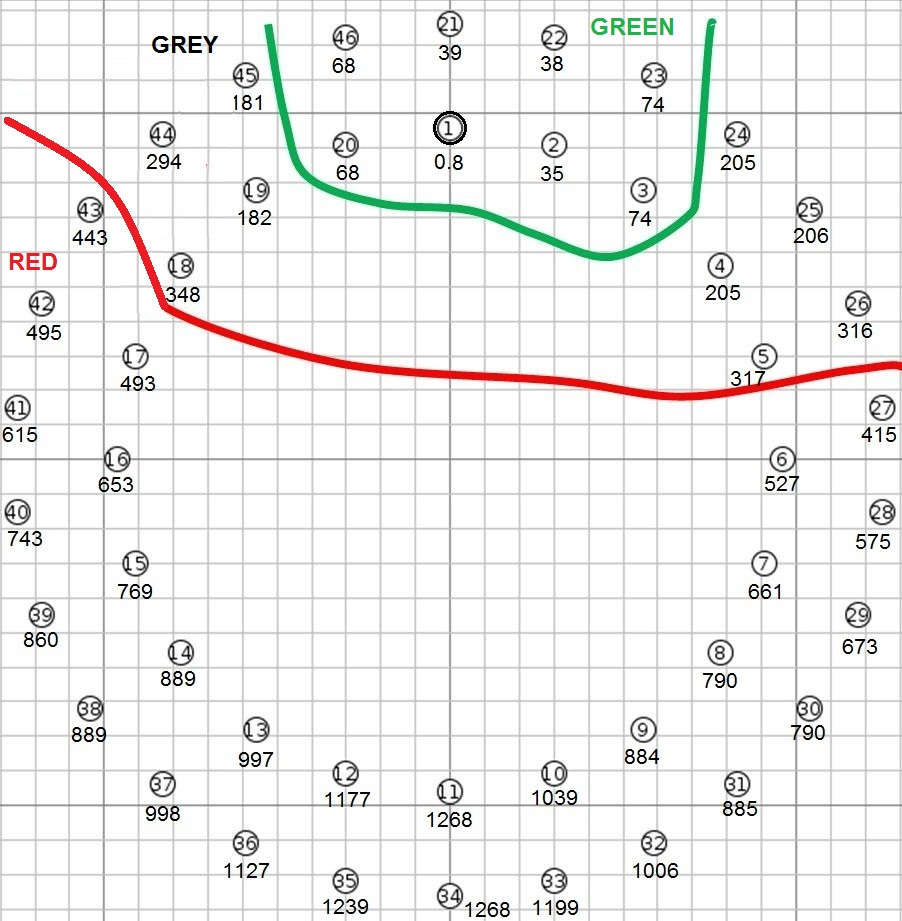
\includegraphics[width=.8\linewidth]{DoubleRingZ}
        \caption{IWS and placement of nodes in Double Ring Topology}
        \label{fig:elliptopo} 
    \end{figure}

Figure~\ref{fig:elliptopo} shows the placement of the motes with mote ID written at the centre and IWS beneath the tiny circle.
The motes represented an intrusion point in the process of measuring IWS using Equation~\ref{eqn2}.
The IWS increases linearly with the increase in distance from the sink.
If IWS in a network are organised in a specific order, it would represent the original topology in some fashion.
For example, in the double ring topology, the circles are represented by the bimodal curve formed from the IWS represented by columns in Figure~\ref{fig:ellipgraph}.
\begin{figure}[tbph!]
	\centering
        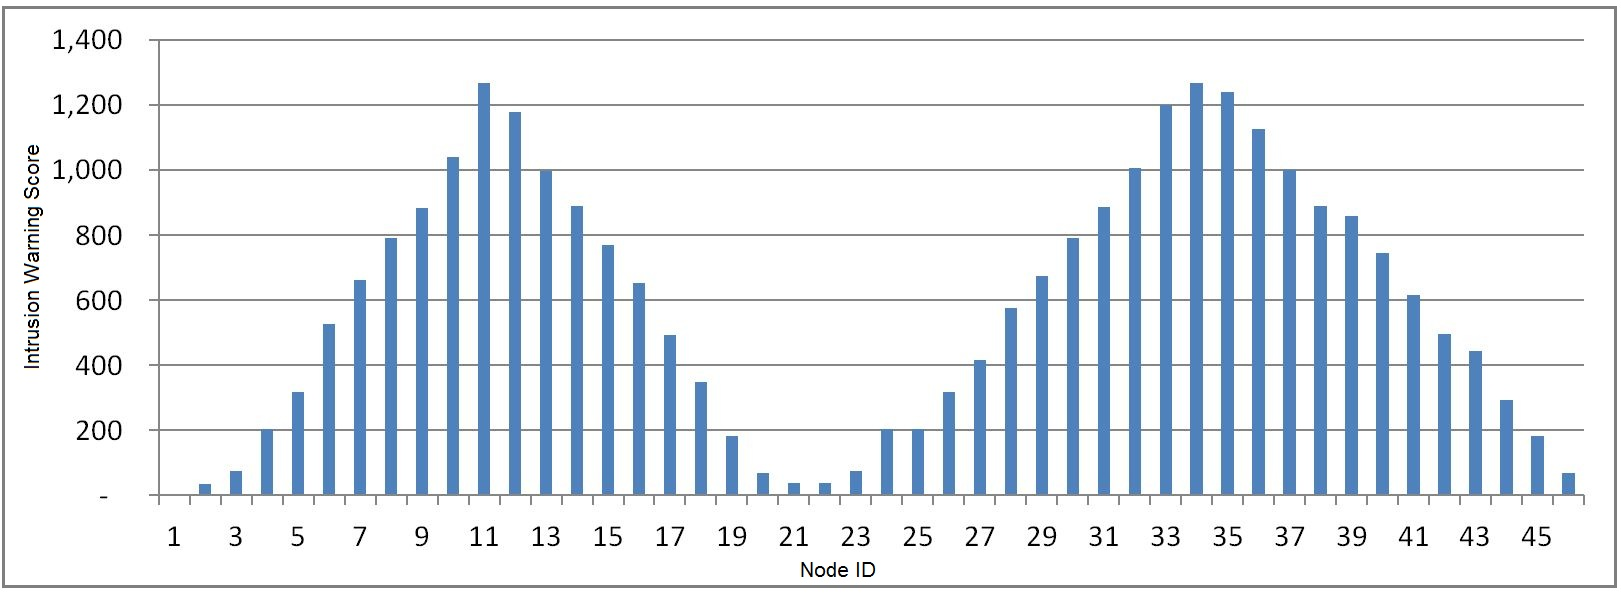
\includegraphics[width=\linewidth]{DR_Column}
        \caption{Comparison of IWS at different motes}
        \label{fig:ellipgraph}
\end{figure}

The main contribution of this research comes from the ability to report anomaly in quantitative term like the IWS.
For example:  a regular legitimate update, initiated from node ID 1, resulted into a IWS of 0.8.
The result matched the theoretical expectation of very low IWS.
In addition to this, for intrusion scenario simulated from the nodes near the sink, the IWS was still fairly low (e.g. at mote ID 2, 3, 20--23, and 46). 
Because IWS of the motes close to the sink are likely to be very low, it is quite difficult to conclude if such an IWS indicate an intrusion.
This area is marked as GREEN zone, and need to be adequately secured with additional physical security as intrusion in these motes are not detectable by the IDS.
For other motes, such as mote ID 4, 5, 24--26, 18, 19, 44 and 45, the IWS is neither too low, nor too high to be considered intrusion. The area is marked as GREY to indicate requirement of additional monitoring to aid false positive cases.
However, for the distant motes--marked in RED zone, the IWS is quite high and the IDS can conclude such cases as intrusion, such as IWS of 1268 for mote ID 34, 885 for mote ID 31,and likewise indicate intrusion.
Accordingly, the Figure~\ref{fig:elliptopo} and~\ref{fig:ellipgraph} shows the region boundaries and thresholds of GREEN, GREY and RED zones.%

\begin{table*}[t]
\centering
\begin{tabular}{|l|*{17}{r|}r|}
\hline
\bd{Node ID}           & \bd{1} & \bd{4} & \bd{10} & \bd{12} & \bd{13} & \bd{15} & \bd{16} & \bd{18} & \bd{27} & \bd{31} & \bd{34} & \bd{36} & \bd{37} & \bd{38} & \bd{39} & \bd{40} & \bd{41} & \bd{44}\\
%Mote ID           & 1 & 2 & 3 & 4 & 5  & 6 & 7 & 8 & 9 & 10 & 11 & 12 & 13 & 14 & 15  & 16 & 17 & 18 & 19 & 20 \\
\hline
\bd{Update Time}  &   404 	&  588 	& 170 	& 66 	& 16 &	 16 	& 65 &	 204 &	 526 & 329 &	 113 &	 66 &	 15 	& 16 	& 16 &	 65 &	125 & 277 \\
\hline
\end{tabular}
\caption{Update Time of motes when intrusion initiated from node 14 in double-ring topology (Data from other node omitted) }
\label{tab:dr_time_14}
\end{table*}

\begin{table*}[t!]
\centering
\begin{tabular}{|l|*{20}{r|}r|}
\hline
\bd{Node ID}           & \bd{1} & \bd{2} & \bd{3} & \bd{4} & \bd{5} & \bd{6} & \bd{7} & \bd{8} & \bd{9} & \bd{10} & \bd{11} & \bd{...} & \bd{33} & \bd{34} & \bd{35} & \bd{36} & \bd{37} & \bd{38} \\
%Mote ID           & 1 & 2 & 3 & 4 & 5  & 6 & 7 & 8 & 9 & 10 & 11 & ...& 31 & 32 & 33  & 34 & 35 & 36 & 37 & 38 \\
\hline		\hline

Power 100\%	   & 512 & 529 & 512 & 512 & 512  & 512 & 476 & 478 & 476 & 459 & 458 & ...& 53  & 48 & 49 & 51 & 47 & 29 \\
\hline

Power 50\%	  &31 & 59&254& 31& 31 &283& 32& 32& 254& 31 &253 & ... & 31  & 30 & 31 & 31 & 30 & 0 \\
\hline
\end{tabular}
\caption{IWS from intrusion at motes in Owheo WSN. Further explained in Figure~\ref{subfig:owheo_full} and~\ref{subfig:owheo_half} }
\label{tab:owheo}
\end{table*}


The IDS can also detect the source of intrusion by analysing update time of all motes. %and its extent. 
For example, Table~\ref{tab:dr_time_14} shows the update time recorded at different motes when intrusion was initiated from note 14.
The timing data shows that lowest timing was recorded at node 13, 15, 37, 38, and 39 which was $\approx$16 seconds.
Node 14 did not report any time because of three reasons: 
\begin{inparaenum}
\item node 14 initiated the update, so it was updated at $0$ second;
\item it acted as a sink, the protocol did not require it to notify update time; and 
\item it is the compromised node whose protocol is expected to be altered.
\end{inparaenum}
From the timing data, the IDS can conclude that node 14 was the intrusion point.
The extent of intrusion, as specified earlier, is found out from reported version information.


%The idea of zoning associated with the IWS is very beneficial in securing a WSN.
The idea of zoning associated with IWS is useful in designing secure WSN deployment, which is considered to be another major contribution of the work.
A network is more secure when it has a smaller GREEN and GREY zone, which implies the requirement of lesser resources to impenetrably secure less number of motes.
%Similarly, a smaller or non-existent GREY zone would require lesser monitoring measures.
%Such a secure WSN can be designed by varying the parameters like power level or even by physically relocating some motes.
Obtaining real world scenario by varying different sets of design parameters such as power levels or position of nodes is an impossible task even for a small WSN.
The simulation environment used to design IDS can be effectively utilised to obtain expected IWS score range for different sets of parameters and then rank the sets based on how effectively they produce IWS values. 
However, any change in topology or design parameters, like power level, will require recalibrating the IDS. 
For example, we have simulated the IWS scenario of the `Owheo Sensor Network' 
at two different power levels in our quest to design a secure WSN using the IDS.

Table~\ref{tab:owheo} shows the IWS at different motes of Owheo WSN as intrusion points at 100\% and 50\% power levels. 
%Here, mote ID 38 was marked as the sink.
At 100\% power level, %19 nodes were in GREEN zone, only one node in GREY zone and the rest 
only 16 nodes were in RED zone.
When the same deployment was simulated at 50\% power level, %only seven nodes were in GREEN zone, two nodes were in GREY zone and rest 
27 motes were in RED zone.
The deployment and the zoning boundaries at 100\% and  50\% power level has been shown in Figure~\ref{subfig:owheo_full} and~\ref{subfig:owheo_half} respectively.
Comparing the scenarios, it can clearly be established that deployment at 50\% power level is more secure than the other because of two reasons:
\begin{inparaenum}
\item it has a smaller sized GREEN and GREY zone; and 
\item there are fewer nodes in these zones. 
\end{inparaenum}

\begin{figure}[tbph!]
	\centering
        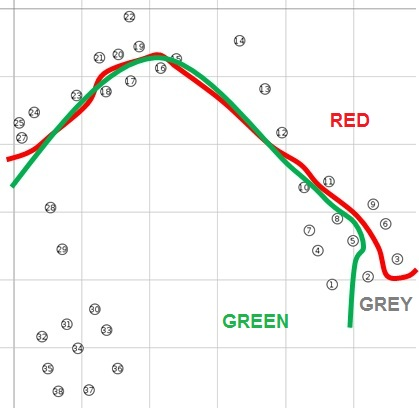
\includegraphics[width=.9\linewidth]{Owheo_full}
        \caption{Zone boundary at Full Power Level}
        \label{subfig:owheo_full}
\end{figure}

\begin{figure}[tbph!]
	\centering
        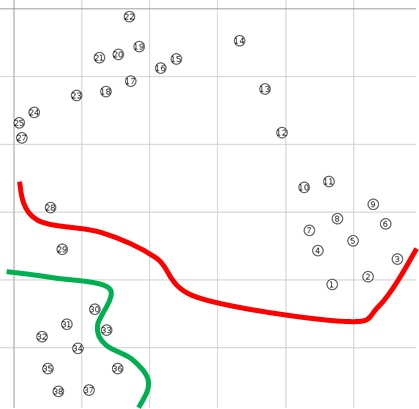
\includegraphics[width=.9\linewidth]{Owheo_half}
        \caption{Zone boundary at Half Power Level}
        \label{subfig:owheo_half}
\end{figure}



%\begin{figure*}[t!]
%    \centering
%    \begin{subfigure}[b]{0.5\textwidth}
%        \centering
%        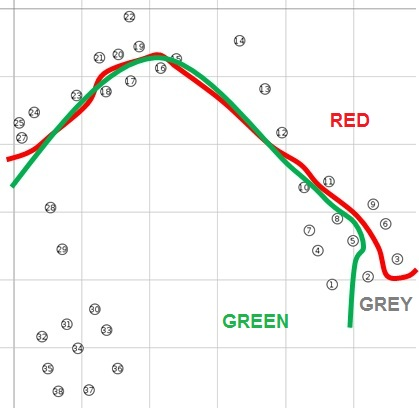
\includegraphics[height=2.5in]{Owheo_full}
%        \caption{Zone boundary at Full Power Level}
%        \label{subfig:owheo_full}
%    \end{subfigure}%
%    ~ 
%    \begin{subfigure}[b]{0.5\textwidth}
%        \centering
%        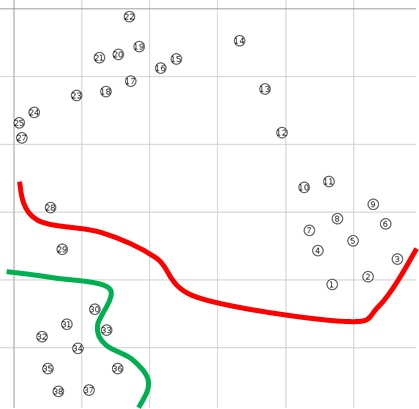
\includegraphics[height=2.5in]{Owheo_half}
%        \caption{Zone boundary at Half Power Level}
%        \label{subfig:owheo_half}
%    \end{subfigure}
%    \caption{Comparison of Zone boundary for power level variations in `Owheo Sensor Network'. IWS of the motes at the power levels are shown in Table~\ref{tab:owheo}}
%\label{fig:owheo}
%\end{figure*}


\section{Conclusion}
\label{sec:concl}

In this paper, we modelled an IDS solution to intrusion in WSN software update protocols.
We discussed the potential danger that is associated with WSN OTA software update.
The IDS is hosted on a server that remains physically connected to the  sink. 
% The sink has an ITC application which in coordination with the IDS performs the detection activity.
% <dme> ITC needs to be explained if included in the conclusion. Doesn't seem high value though.
The system watches over the timing of software update patterns using a modified version of the Deluge protocol.
%Whenever a mote is updated, it sends an update related information to designated sink using a datagram.  
%Related information from the datagram is filtered by the ITC for further processing at IDS.

The first contribution of the research is quantifying intrusion through an IWS that indicates the location and extent of intrusion.
%The IWS is a quantitative indicator of possible intrusion.
%The utility function that computes IWS is designed to neutralise the undesired %/unexpected
%changes in mean and standard deviation which are expected to contribute to a near zero IWS.
The other important contribution is related to designing secure WSN using IWZ.
%classifying expected IWS into zones.
%The concept of zoning using the IDS is a very useful tool in designing secure WSN deployment.
%The IDS can be used to simulate all possible combinations of parameters and  to rank the sets based on intrusion vulnerability.
%For example, a WSN with known small insecure zone is much easier to protect than a larger zone.
%The ranking mechanism is useful in such scenario.
Besides, the IDS also can indicate some other kinds of anomalies such as node relocation, node repudiation or node compromise.

The IDS has several limitations. 
It assumes some special cases like a static WSN with a single sink.
It also assumes that network-wide information will not be forged. %to have network wide transparent knowledge.
These assumptions may not hold in a real WSN.
In addition to this, assumptions about the attacker are: the attacker can employ enough resources to break in the cryptographic protections in sensors; however, he is not able to modify the protocols in an uncompromised sensor.
The IDS has an obvious functional limitation.
It cannot identify an intrusion in certain scenarios such as 
%For example, when an intrusion takes place 
in close vicinity of the sink.%, this IWS may not always be sufficiently large to be identified as an intrusion.
The other limitation stems from the fact that the results are based on simulated data and need support from real world implementation.
In future,  the IDS can be implemented to examine real world performance including cases of multiple sinks with mobile sensors.


% \section{References}
% References should be in the standard author-date format, examples of which are shown below (shown is a conference paper, a thesis, a book, a book section and a journal paper in that order).  The required formats can be obtained by including the {\it natbib} package and using style {\it agsm}.  The files {\tt natbib.sty} and {\tt agsm.bst} are available at the CRPIT website.  The  {\it harvard} package, which is also available, can also be used as an alternative to natbib.

\bibliographystyle{agsm}    % or some other suitable package.
\bibliography{auspdc}
%\bibliography{CRPITExample}  % often included from a separate file.

% \begin{thebibliography}{xx}

% \harvarditem[Agrawal et~al.]{Agrawal, Imielinski \harvardand\
  % Swami}{1993}{AIS93}
% Agrawal, R., Imielinski, T. \harvardand\ Swami, A.  \harvardyearleft
  % 1993\harvardyearright , Mining association rules between sets of items in
  % large databases, {\em in} `ACM SIGMOD International Conference on Management
  % of Data', Vol.~22, ACM Press, Washington DC, USA, pp.~207--216.

% \harvarditem{Ben-Zvi}{1982}{BenZvi82}
% Ben-Zvi, J.  \harvardyearleft 1982\harvardyearright , The time relational
  % model, Ph.{D}., University of California, Los Angeles.

% \harvarditem{Bentley}{1986}{Bentley86}
% Bentley, J.  \harvardyearleft 1986\harvardyearright , {\em Programming pearls},
  % Addison-Wesley.

% \harvarditem[Fayyad et~al.]{Fayyad, Piatetsky-Shapiro \harvardand\
  % Smyth}{1996}{FPS96}
% Fayyad, U.~M., Piatetsky-Shapiro, G. \harvardand\ Smyth, P.  \harvardyearleft
  % 1996\harvardyearright , From data mining to knowledge discovery: An overview,
  % {\em in} U.~Fayyad, G.~Piatetsky-Shapiro, P.~Smyth \harvardand\
  % R.~Uthurusamy, eds, `Advances in Knowledge Discovery and Data Mining', AAAI
  % Press/ MIT Press, pp.~1--34.

% \harvarditem{Snodgrass}{1987}{Snodgrass87}
% Snodgrass, R.  \harvardyearleft 1987\harvardyearright , `The temporal query
  % language tquel', {\em ACM Transactions on Database Systems} {\bf
  % 12}(2),~247--298.

% \end{thebibliography}


\end{document}

